
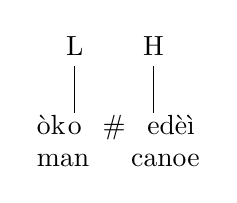
\begin{tikzpicture}
		\node (s1)[anchor=base] at (-.3, 0) {òk} ; 
        \node (s1)[anchor=base] at (0, 0) {o} ; 
		\node (gl1)[anchor=base] at (-.15, -.4) {man} ; 
		\node (wb)[anchor=base] at (0.5, 0) {\#} ; 
		\node (s2)[anchor=base] at (1, 0) {e} ; 
		\node (ss)[anchor=base] at (1.3, 0) {dèì} ; 
		\node (gl1)[anchor=base] at (1.15, -.4) {canoe} ; 
        \node[anchor=base] (t1) at (0,1) {L} ; 
        \node[anchor=base] (t2) at (1,1) {H} ;
	\draw (s1) -- (t1) ;
	\draw (s2) -- (t2) ;
\end{tikzpicture}
\hfill
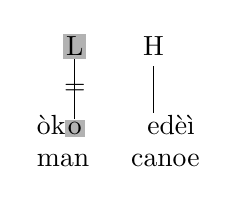
\begin{tikzpicture}
% grey highlight FIRST (so it stays behind)
% \fill[gray!20] (-0.15,-0.2) rectangle (0.3,1.5);
\node (s1a)[anchor=base] at (-.3, 0) {òk} ; 
\node (s1)[anchor=base, fill=black!30, inner sep=1pt] at (0, 0) {o};
\node (gl1)[anchor=base] at (-.15, -.4) {man} ; 
% \node (wb)[anchor=base] at (0.5, 0) {\#} ; 
\node (s2)[anchor=base] at (1, 0) {e} ; 
\node (ss)[anchor=base] at (1.3, 0) {dèì} ; 
\node (gl2)[anchor=base] at (1.15, -.4) {canoe} ; 

\node[anchor=base, fill=black!30, inner sep=1pt](t1) at (0,1) {L} ; 
\node[anchor=base] (t2) at (1,1) {H} ;

\draw (s1) -- (t1) node[midway] {$=$} ;
\draw (s2) -- (t2) ;
\end{tikzpicture}
\hfill
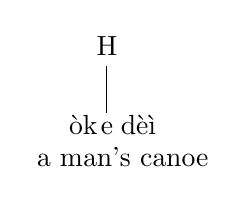
\begin{tikzpicture}
		\node (s1)[anchor=base] at (0, 0) {òk} ; 
        % \node (s1)[anchor=base] at (0, 0) {o} ; 
		\node (gl1)[anchor=base] at (.5, -.4) {a man's canoe} ; 
		\node (s2)[anchor=base] at (.3, 0) {e} ; 
		\node (ss)[anchor=base] at (.7, 0) {dèì} ; 
		% \node (gl1)[anchor=base] at (1.15, -.4) {canoe} ; 
        % \node[anchor=base] (t1) at (0,1) {L} ; 
        \node[anchor=base] (t2) at (.3,1) {H} ;
	% \draw (s1)[dotted] -- (t1) ;
	\draw (s2) -- (t2) ;
\end{tikzpicture}

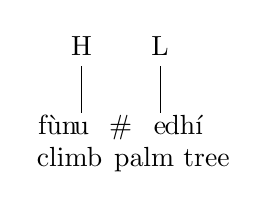
\begin{tikzpicture}
		\node (s1)[anchor=base] at (-.3, 0) {fùn} ; 
        \node (s1)[anchor=base] at (0, 0) {u} ; 
		\node (gl1)[anchor=base] at (-.15, -.4) {climb} ; 
		\node (wb)[anchor=base] at (0.5, 0) {\#} ; 
		\node (s2)[anchor=base] at (1, 0) {e} ; 
		\node (ss)[anchor=base] at (1.3, 0) {dhí} ; 
		\node (gl1)[anchor=base] at (1.15, -.4) {palm tree} ; 
        \node[anchor=base] (t1) at (0,1) {H} ; 
        \node[anchor=base] (t2) at (1,1) {L} ;
	\draw (s1) -- (t1) ;
	\draw (s2) -- (t2) ;
\end{tikzpicture}
\hfill
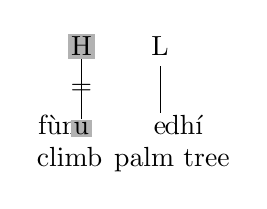
\begin{tikzpicture}
% grey highlight FIRST (so it stays behind)
% \fill[gray!20] (-0.15,-0.2) rectangle (0.3,1.5);
		\node (s1)[anchor=base] at (-.3, 0) {fùn} ; 
\node (s1)[anchor=base, fill=black!30, inner sep=1pt] at (0, 0) {u};
		\node (gl1)[anchor=base] at (-.15, -.4) {climb} ; 
% \node (wb)[anchor=base] at (0.5, 0) {\#} ; 
\node (s2)[anchor=base] at (1, 0) {e} ; 
\node (ss)[anchor=base] at (1.3, 0) {dhí} ; 
\node (gl2)[anchor=base] at (1.15, -.4) {palm tree} ; 

\node[anchor=base, fill=black!30, inner sep=1pt](t1) at (0,1) {H} ; 
\node[anchor=base] (t2) at (1,1) {L} ;

\draw (s1) -- (t1) node[midway] {$=$} ;
\draw (s2) -- (t2) ;
\end{tikzpicture}
\hfill
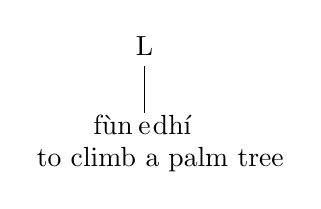
\begin{tikzpicture}
		\node (s1)[anchor=base] at (-.1, 0) {fùn} ; 
        % \node (s1)[anchor=base] at (0, 0) {o} ; 
		\node (gl1)[anchor=base] at (.5, -.4) {to climb a palm tree} ; 
		\node (s2)[anchor=base] at (.3, 0) {e} ; 
		\node (ss)[anchor=base] at (.65, 0) {dhí} ; 
%		\node (gl2)[anchor=base] at (1.15, -.4) {palm tree} ; 
		% \node (gl1)[anchor=base] at (1.15, -.4) {canoe} ; 
        % \node[anchor=base] (t1) at (0,1) {L} ; 
        \node[anchor=base] (t2) at (.3,1) {L} ;
	% \draw (s1)[dotted] -- (t1) ;
	\draw (s2) -- (t2) ;
\end{tikzpicture}